\documentclass[10pt,a4paper,oneside,titlepage]{article}
\usepackage[utf8]{inputenc}
\usepackage[english,russian]{babel}
\usepackage{amsmath}
\usepackage{amsthm}
\usepackage{amssymb}
\usepackage{cmll}
\usepackage{enumerate}
\usepackage{stmaryrd}
\usepackage[left=2cm,right=2cm,top=2cm,bottom=2cm,bindingoffset=0cm]{geometry}
\usepackage{url}
\usepackage{listingsutf8}
\usepackage{graphicx}
\graphicspath{{pictures/}}
\DeclareGraphicsExtensions{.pdf,.png,.jpg}

\lstset{%
	numbers = left
}

\title{Конспект по курсу Паралелльное программирование \thanks{Читаемый Романом Елизаровым  Никитой Ковалем в 2018-2019 годах}}
\author{Александра Лисицына \thanks{Студентка группы М3334}}

\theoremstyle{plain}
\newtheorem{theorem}{Теорема}[section]
\newtheorem{lemma}{Лемма}[section]

\theoremstyle{defenition}
\newtheorem*{defenition}{Определение}

\begin{document}
	
\maketitle

\tableofcontents

\clearpage	
\section{Intoduction}
\subsection{Закон Мура}
Каждые 2 года количество транзисторов на процессоре удваивается.
До, примерно, 2005 года также росла частота ядра. Также начал замедляться рост производительность ядра. С 2005 года начался рост числа ядер.

\includegraphics*[scale=0.5]{Mura1}

\includegraphics*[scale=0.5]{Mura2}

\includegraphics*[scale=0.5]{Mura3}

\includegraphics*[scale=0.5]{Mura4}

\begin{defenition}
	{\bfseries Масштабирование} - свойство системы выполнять больше действий при увеличении мощности(традиционное), количества ядер(многопоточное).
\end{defenition}

В реале не получается сделать все идеально и для этого нужно изучать многопоточное программирование.

\subsection{Закон Амдала}
$$
S=\frac{Время на 1 ядре}{Время на N ядрах}
$$
где $S$ - это ускорение кода

Или
$$
S=\frac{1}{1-P+P/N}
$$
где $P$ - доля параллельного кода

Максимальное ускорение кода достигается при $N\to \infty$ и равно $1/(1-P)$

\begin{tabular}{cc}
	$P$&$S$\\[5pt]
	60\%&2.5\\
	95\%&20\\
	99\%&100\\
\end{tabular}

Поэтому нам необходимо увеличивать долю параллельного кода для достижения наилучшей масштабируемости.

\subsection{Разные виды параллелизма}
\subsubsection{Параллелизм на уровне инструкций (ILP)}\footnotetext{Instuction Level Parallelism}
Способы использования ILP

\begin{itemize}
	\item Конвейер
	
	\item Суперскалярное исполнение\footnote{Несколько операций за такт}
	
	\begin{itemize}
		\item Внеочередное исполнение
		
		\item Переименование регистров\footnote{Чтобы не возникало ложной зависимости по регистрам}
		
		\item Спекулятивное исполнение\footnote{Начинает выполнять одну из веток перехода, пытаясь ее предсказать}
		
		\item Предсказание переходов
	\end{itemize}

    \item Длинное машинное слово (VLIW\footnote{Very Long Instuction Word})
    
    \item Векторизация (SIMD)
\end{itemize}

\begin{figure}[h]
	\centering
	\includegraphics*[width=0.7\linewidth]{pictures/Processors}
	\caption{}
	\label{fig:processors}
\end{figure}

У параллелизма на уровне инструкций есть предел, поэтому нам необходимо параллельное программирование

\paragraph{Симметричная мультипроцессорность (SMP)}\footnotetext{Symmetric Multiprocessing}

Несколько вычислительных ядер у каждого свой поток исполняемых ресурсов

\begin{figure}[h]
	\centering
	\includegraphics*[width=0.4\linewidth]{pictures/SMP}
	\caption{SMP}
	\label{fig:smp}
\end{figure}



\paragraph{Одновременная многозадачность (SMT)}\footnotetext{Simultaneous Multithreading}

Два или более потока одновременно исполняются одним физическим ядром. Снаружи выглядит как SMP.

\begin{figure}[h]
	\centering
	\includegraphics*[width=0.4\linewidth]{pictures/SMT}
	\caption{SMT}
	\label{fig:smt}
\end{figure}



\paragraph{Ассимметричный доступ к памяти (NUMA)}\footnotetext{Non-uniform memory access}

Модель программирования та же, что в SMP, но без общей памяти.

\begin{figure}[h]
	\centering
	\includegraphics*[width=0.4\linewidth]{pictures/NUMA}
	\caption{NUMA}
	\label{fig:numa}
\end{figure}

\subsection{Операционные системы}
\begin{itemize}
	\item Типы
	\begin{itemize}
		\item Однозадачные
		\item Системы с пакетными задачами (batch processing)
		\item Многозадачные / с разделением времени (time sharing)
		\begin{itemize}
			\item Кооперативная многозадачность (cooperative multitasking)
			\item Вытесняющая многозадачность (preemptive multitasking)
		\end{itemize}
	\end{itemize}
    \item История многозадчности
    \begin{itemize}
    	\item Изначально нужно было для раздела одной дорогой машины между несколькими пользователями
    	\item Теперь нужно для использования ресурсов одной многоядерной машины для множества задач
    \end{itemize}
\end{itemize}

\subsection{Основные понятия в современных ОС}
\begin{itemize}
	\item \begin{defenition}
		{\bfseries Процесс} --- владеет памятью и ресурсами.
	\end{defenition}
	\item \begin{defenition}
		{\bfseries Поток} --- контекст исполнения внутри процесса.
	\end{defenition}
	\begin{itemize}
		\item В одном процессе может быть несколько потоков
		\item Все потоки работают с общей памятью процесса
	\end{itemize}
    \item Но в теории мы их будем смешивать
\end{itemize}

\subsection{Формализм}
\subsubsection{Модели программирования}
\begin{itemize}
	\item <<Классическое>> однопоточное / однозадачное
	\begin{itemize}
		\item Можем использовать ресурсы многоядерной системы только запустив несколько независимых задач
	\end{itemize}
    \item Многозадачное программирование
    \begin{itemize}
    	\item Возможность использовать ресурсы многоядерной системы в рамках решения одной задачи
    	\item Варианты:
    	\begin{itemize}
    		\item Модель с общей памятью
    		\item Модель с передачей сообщений (распределенное программирование)
    	\end{itemize}
    \end{itemize}
\end{itemize}

\begin{figure}[h]
	\centering
	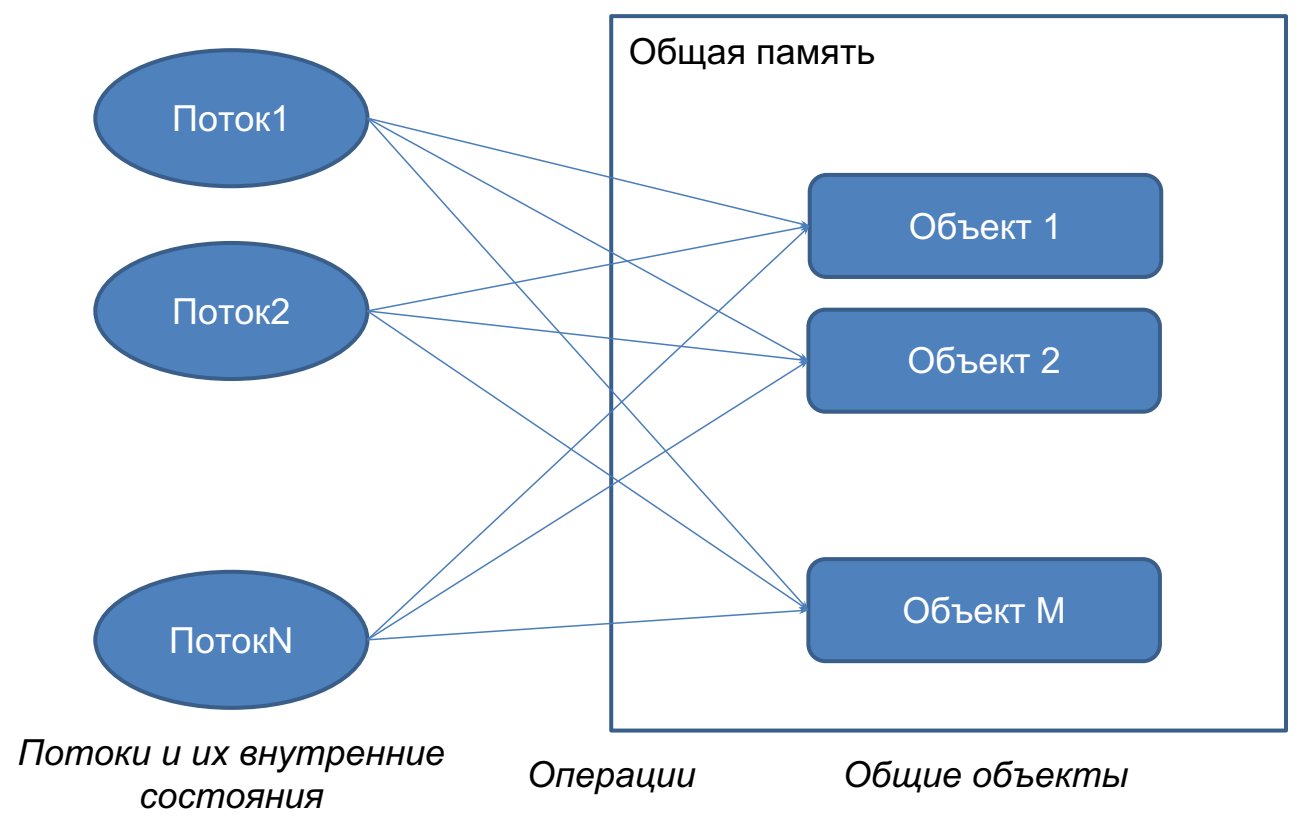
\includegraphics[width=0.7\linewidth]{pictures/CommonMemory}
	\caption{Модель с общими объектами (общей памятью)}
	\label{fig:commonmemory}
\end{figure}

\subsubsection{Общие объекты}
\begin{itemize}
	\item Потоки выполняют операции над общими, разделемыми объектами
	\item В этой моделе не важны операции внутри потоков
	\item Важна только коммуникация между потоками
	\item В этой моделе единственный тип коммуникации между потоками --- это работа с общими объектами
\end{itemize}

\subsubsection{Общие переменные}
\begin{itemize}
	\item Общие переменные --- это простейший тип общего объекта:
	\begin{itemize}
		\item У него есть значение определенного типа
		\item Есть операция чтения (read) и записи (write)
	\end{itemize}
    \item Общие переменные --- это базовые строительные блоки для многопоточных алгоритмов
    \item Модель с общими переменными --- это хорошая абстракция современных многопроцессорных систем и многопоточных ОС
    \begin{itemize}
    	\item На практике, это область памяти процесса, которая одновременно доступна для чтения и записи всем потокам этого процесса
    \end{itemize}
\end{itemize}

В теоретических трудах общие переменные называют регистрами

\subsubsection{Свойства многопоточных программ}
\begin{itemize}
	\item Последовательные программы детерминированы
	\begin{itemize}
		\item Если нет использования случайных чисел и другого явного общения с недетеминированным миром
		\item Их свойства можно установить анализируя последовательное исполнение при данных входных параметрах
	\end{itemize}
    \item Многопоточные программы в общем случае недетерминированы
    \begin{itemize}
    	\item Даже если код каждого потока детерминирован
    	\item Результат работы зависит от фактичекого исполнения при данных входных параметрах
    	\item А этих исполнений может быть много
    \end{itemize}
    \item Говорим <<Программа A имеет свойство P>> если она имеет это свойство при любом исполнении
\end{itemize}

\subsubsection{Моделирование многопотчного исполнения}

\begin{center}
	\begin{lstlisting}
	shared int x = 0, y = 0
	\end{lstlisting}
\end{center}
	
	\begin{minipage}{0.4\textwidth}
		Thread P:
		
		\begin{lstlisting}
		x = 1
		r1 = y
		stop
		\end{lstlisting}
	\end{minipage}
	\hfill
	\begin{minipage}{0.4\textwidth}
		Thread Q:
		
		\begin{lstlisting}
		y = 1
		r2 = x
		stop
		\end{lstlisting}
	\end{minipage}

\paragraph{Моделирование исполнений через чередование операций}

\begin{figure}[h!]
	\centering
	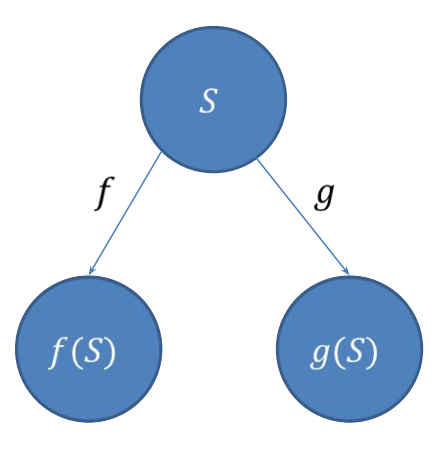
\includegraphics[width=0.3\linewidth]{pictures/Model}
	\caption{}
	\label{fig:model}
\end{figure}

\begin{itemize}
	\item $S$ --- это общее состояние:
	\begin{itemize}
		\item Состояние всех потоков (IP+locals)
		\item И состояние всех общих объектов
	\end{itemize}
    \item $f$ и $g$ --- это операции
    \begin{itemize}
    	\item Количество различных операций в каждом состоянии равно количеству потоков
    \end{itemize}
    \item $f(S)$ --- это новое состояние после применения операции $f$ к состоянию $S$ 
\end{itemize}

\begin{figure}[h!]
	\centering
	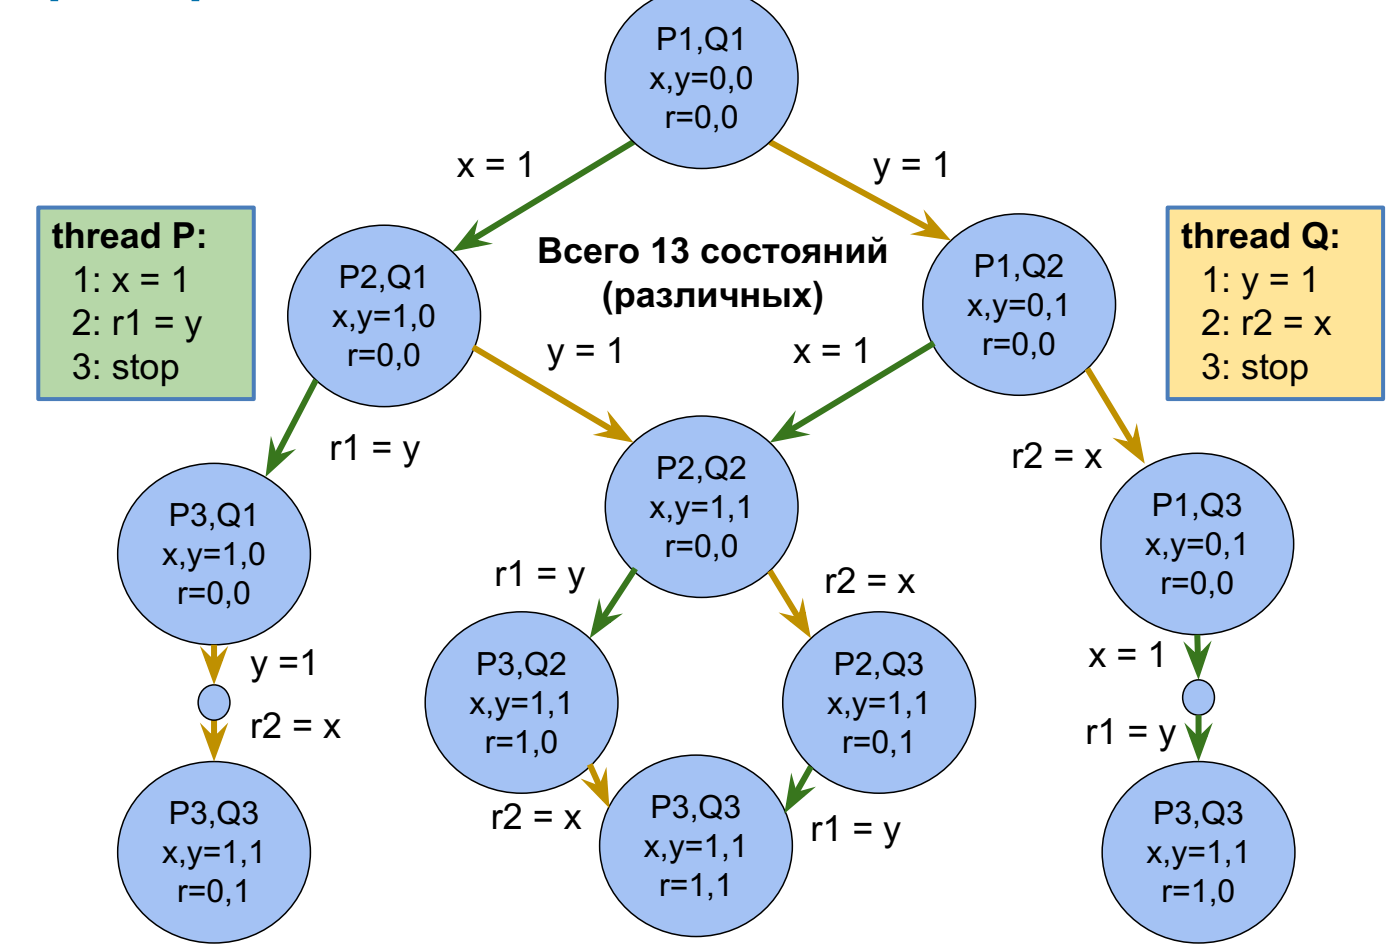
\includegraphics[width=0.5\linewidth]{pictures/Model1}
	\caption{}
	\label{fig:model1}
\end{figure}


После исполнеия этого кода для r1, r2 возможны следующие пары значений: (0, 0), (0, 1), (1, 0), (1, 1). Хотя при моделировании через чередование (рисунок~\ref{fig:model1}) первого варианта не получается. Это случается, так как в современном процессоре запись не попадает сразу в общую память, а в начале буферизируется (т.к. запись долгая операция). Поэтому мы можем прочитать старое значение, т.к. чтение быстрая операция и новые значения еще лежат в буфере. Процессор может переставить инструкции, т.к. это может ускорить однопоточный код (процессро не знает о параллельности).

\begin{figure}[h!]
	\centering
	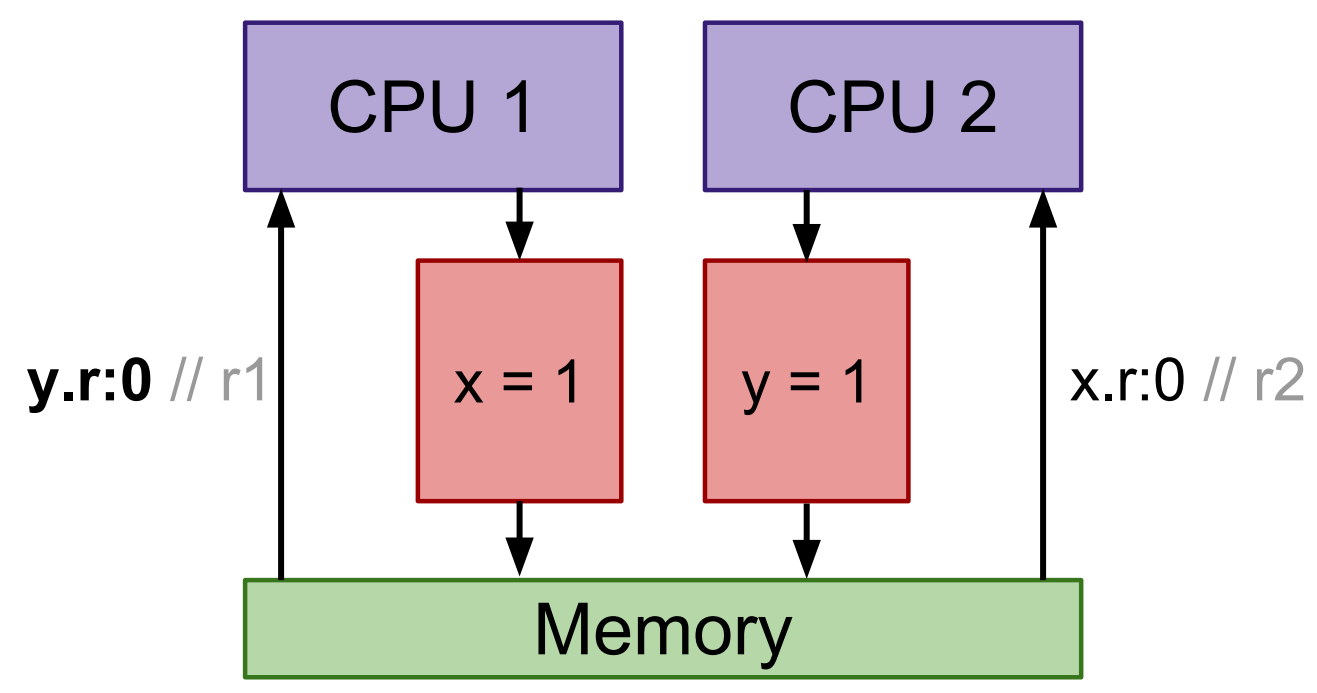
\includegraphics[width=0.4\linewidth]{pictures/Memory}
	\caption{}
	\label{fig:memory}
\end{figure}

Модель чередования не параллельна

На самом деле в настоящих процессорах операции чтения и записи не мгновенные. Они происходят паралелльно как в разных ядрах, так и в одном.

И вообще процессор обменивается с памятью сообщениями о чтении / записи и таких сообщений одновременно в обработке может быть очень много.

\section{Lock-free Treiber Stack and Michael-Scott Queue}

\section{Определения и формализм}
\subsection{Физическая реальность}
\begin{itemize}
	\item Свет (электромагнитные волны) в вакууме распространется со скоростью $\sim3\cdot10^8$ м/с.
	\begin{itemize}
		\item Это максимальный физический предел скорости
		\item За один такт процессора с частотой 3 ГГц ($3\cdot10^9$ Гц) свет в вакууме проходит всего 10 см.
	\end{itemize}
    \item Соседние процессоры физически не могут синхронизировать свою работу и физически не могут определить порядок происходящих в них событиях.
    \begin{itemize}
    	\item Они работают действительно физически параллельно
    \end{itemize}
    \item Пусть $a, b, c\in E$ --- это физически атомарные (неделимые) события, происходящие в пространстве--времени (рисунок~\ref{fig:model2})
    \begin{itemize}
    	\item Говорим <<$a$ предшествует $b$>> или <<$a$ произошло до $b$>> (и записываем $a\to b$), если свет от точки пространства--времени $a$ успевает дойти до точки пространства--времени $b$.
    	\item Это отношение частичного пордка на событиях
    \end{itemize}
\end{itemize}

\begin{figure}[h!]
	\centering
	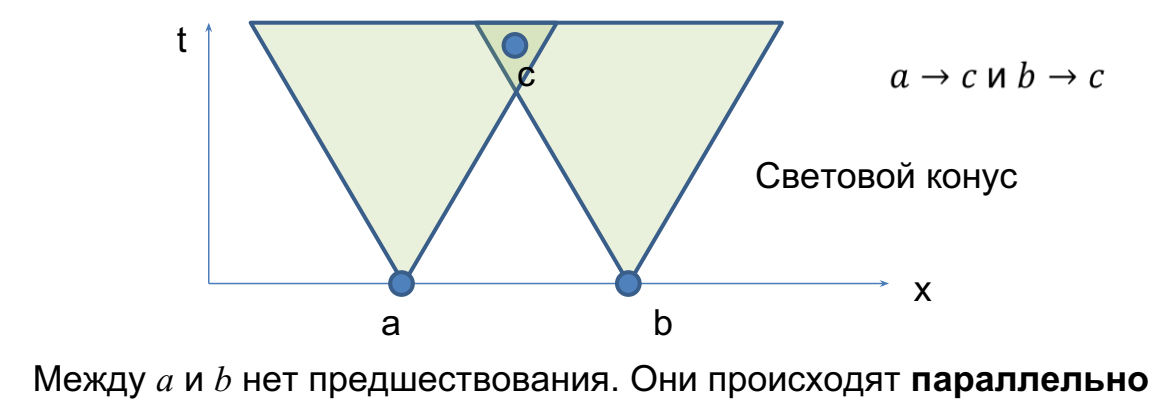
\includegraphics[width=0.5\linewidth]{pictures/Model2}
	\caption{}
	\label{fig:model2}
\end{figure}

\subsection{Модель <<произошло до>> (happens before)}
\begin{itemize}
	\item Впервые введена Л.~Лампортом в 1978 году.
	\item Исполнение системы --- это пара ($H, \to_H$)
	\begin{itemize}
		\item $H$ --- это множество операций $e, f, g, \ldots$ (чтение и запись ячеек памяти и т.~п.) произошедших во время исполнения
		\item $\to_H$ --- это транзитивное, антирефлексивное, ассимметричное отношение (частичный строгий порядок) на множестве операций
		\item $e\to_Hf$ означает, что <<$e$ произошло до $f$ в исполнении $H$>>. Чаще всего исполнение $H$ понятно из контекста и опускается 
	\end{itemize}
    \item Две операции $e$ и $f$ параллельны ($e\parallel f$), если $e\nrightarrow f\wedge f\nrightarrow e$.
    \item Система --- это набор всех возможных исполнений системы
    \item Говорим, что <<система имеет свойство P>>, если каждое исполнение системы имеет свойство P.
\end{itemize}

\subsection{Модель глобального времени}
В этой моделе каждая операция --- это временный интервал (рисунок~\ref{fig:model3}) $e=[t_{inv}(e), t_{res}(e)]$ где $t_{inv}(e), t_{res}(e)\in\mathbb{R}$ и
$$
e\to f\stackrel{\mathrm{def}}{=}t_{res}(e)<t_{inv}(f)
$$

\begin{figure}
	\centering
	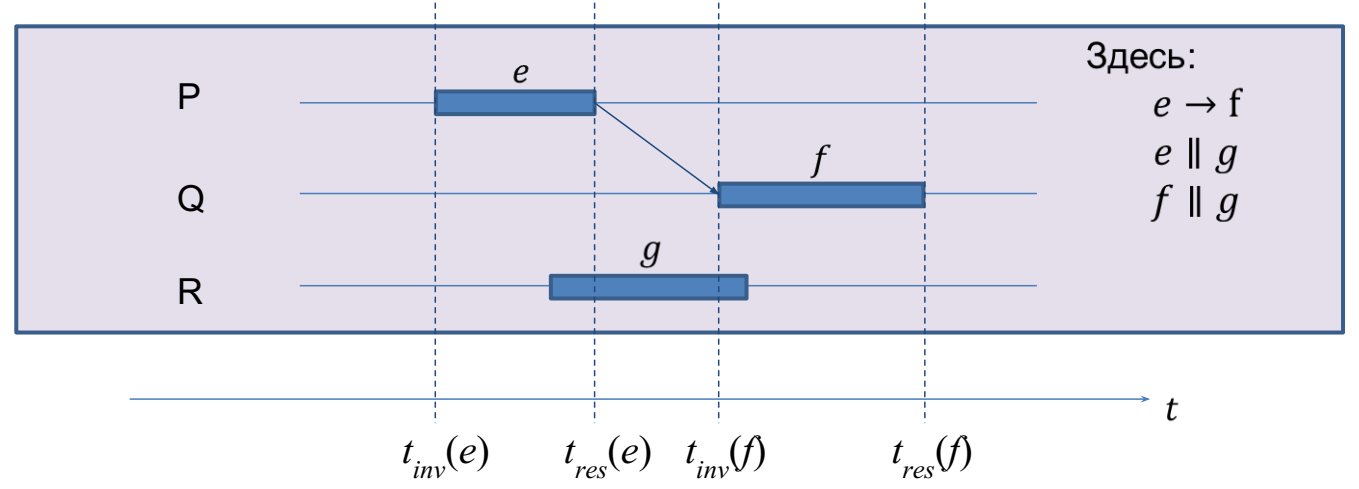
\includegraphics[width=0.5\linewidth]{pictures/Model3}
	\caption{Модель глобального времени}
	\label{fig:model3}
\end{figure}

\subsection{Обсуждение глобального времени}
На самом деле никакого глобального времени нет и не может быть из--за физических ограничений.

\begin{itemize}
	\item Это всего лишь механизм, позволяющий визуализировать факт существования параллельных операций.
	\item При доказательстве различных фактов и анализе свойств [исполнений] системы время не используется
	\begin{itemize}
		\item Анализируютя только операции и отношения <<произошло до>>
	\end{itemize}
\end{itemize}

\subsection{<<Произошло до>> на практике}
\begin{itemize}
	\item Современные языки программирования предоставляют программисту операции синхронизации:
	\begin{itemize}
		\item Специальные механизмы чтения и записи переменных
		\item Создание потоков и ожидание их завершения
		\item Различные другие библиотечные примитивы для синхронизации
	\end{itemize}
    \item Модель памяти языка программирования определяет то, каким образом исполнение операций синхронизации создает отношение <<произошло до>>
    \begin{itemize}
    	\item Без них разные потоки выполняются параллельно
    	\item Можно доказать те или иные свойства многопоточного кода, используя гарантии на возможные исполнения, которые дает модель памяти
    \end{itemize}
\end{itemize}

\subsection{Свойства исполнений над общими объектами}
\subsubsection{Операции над общими объектами}
\begin{figure}[h!]
	\centering
	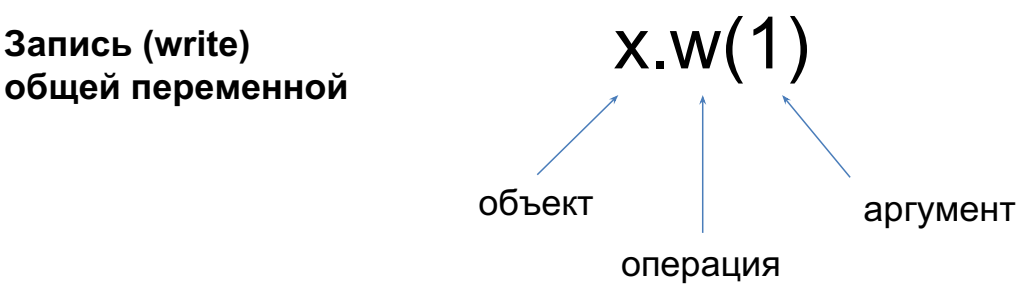
\includegraphics[width=0.6\linewidth]{pictures/Write}
	\caption{Запись}
	\label{fig:write}
\end{figure}

\begin{figure}[h!]
	\centering
	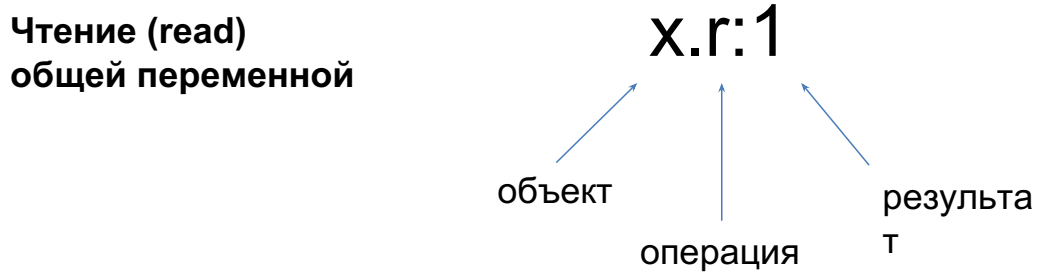
\includegraphics[width=0.6\linewidth]{pictures/Read}
	\caption{Чтение}
	\label{fig:read}
\end{figure}


\subsubsection{Последовательное исполнение}
\begin{defenition}
	Исполнение системы называется последовательным, если все операции линейно--упорядочены отношением <<произошло до>>, то есть $\forall e, f\in H\colon (e=f)\vee(e\to f)\vee(f\to e)$.
\end{defenition}

\begin{figure}
	\centering
	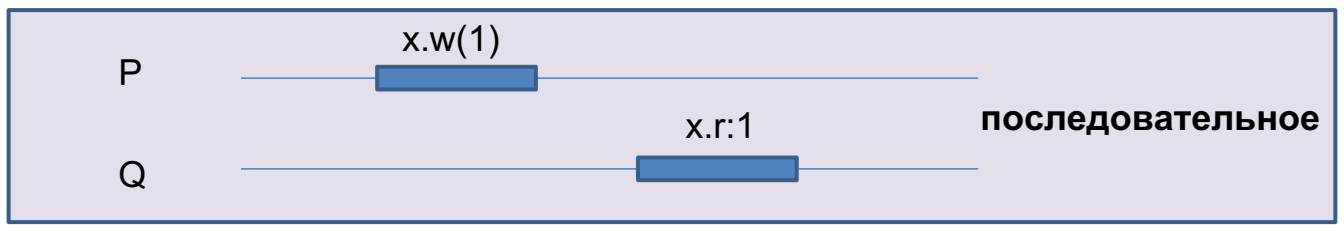
\includegraphics[width=0.4\linewidth]{pictures/Model4}
	\caption{Последовательное исполнение}
	\label{fig:model4}
\end{figure}

\begin{figure}
	\centering
	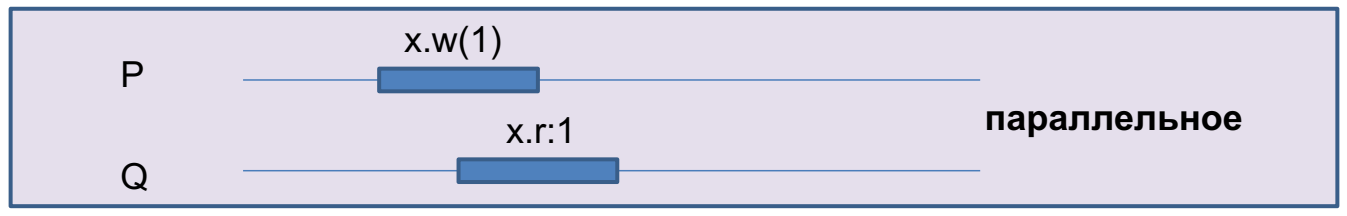
\includegraphics[width=0.4\linewidth]{pictures/Model5}
	\caption{Параллельное исполнение}
	\label{fig:model5}
\end{figure}

\subsubsection{Конфликты и гонки данных (data race)}
\begin{itemize}
	\item \begin{defenition}
		Две операции над одной переменной, одна из которых запись, называются конфликтующими.
	\end{defenition}
    Конфликтующие операции не коммутируют в модели чередования.
	\item \begin{defenition}
		Если две конфликтующие операции произошли параллельно, то такая ситуация называется гонка данных (data race).
	\end{defenition} 
	\begin{itemize}
		\item Это свойство конкретного исполнения.
	\end{itemize}
\end{itemize}

\begin{defenition}
	Программа, в любом допустимом исполнении которой (с точки зрения модели памяти) нет гонок данных, называется корректно синхронизированной.
\end{defenition}

\subsubsection{Правильное исполнение} 


\section{Построение атомарных объектов и блокировки}

\section{Consensus}
\subsection{Задача о консенсусе}

Каждый поток использует объект Consensus один раз

\begin{itemize}
	\item Согласованность: все потоки должны вернуть одно и тоже значение из метода decide
	\item Обоснованность: возвращенное значение было входным значением какого-то из потоков
	\item Без ожидания
\end{itemize}

\subsection{Консенсусное число}
\begin{itemize}
	\item Если с помощью класса атомарных объектов C и атомарных регистров можно реализовать консенсусный протокол без ожидания с помощью детерминированного алгоритма для N потоков (и не больше), то говорят, что у класса C консенсусное число N.
	\item \begin{theorem}
		Атомарные регистры имеют консенсусное число 1.
	\end{theorem} 
\end{itemize}

\subsection{Модель}
\begin{itemize}
	\item x--валентное состояние системы --- консенсус во всех нижестоящих листьях будет x.
	\item Бивалентное состояние --- возможен консенсус как 0, так и 1.
	\item Критическое состояние --- такое бивалентное состояние, у которого все дети одновалентны
\end{itemize}

\subsection{Read--Modify--Write регистры}

\subsection{Универсальность консенсуса}
\begin{theorem}
	Любой последовательный объект можно реализовать без ожидания для N потоков, используя консенсусный проткол для N потоков
\end{theorem}

\section{Алгоритмы без блокировок: Построение на регистрах}
\subsection{Безусловные условия прогресса}
\begin{itemize}
	\item Отсутствие помех --- Если несколько потоков пытаются выполнить операцию, то любой из них должен выполнить ее за конечное время, если все другие остановить в любом месте
	\item Отсутствие блокировки --- если несколько потоков пытаются выполнить операцию, то хотя бы один из них должен выполнить ее за конечное время, независимо от действия или бездействия других потоков
	\item Отсутствие ожидания --- если поток хочет выполнить операцию, то он выполнит ее за конечное время независимо от других потоков
\end{itemize}

\section{CASN}
\subsection{Списки против массивов}
\begin{itemize}
	\item Список
	\begin{itemize}
		\item $3*N$ слов памяти (минимум)
		\item при многопотном использовании хватает одного CAS для добавления элемента
	\end{itemize}
    \item Массив
    \begin{itemize}
    	\item $5+N$ слов памяти (до $5+2*N$ при х2 резерве)
    	\item Как минимум в два раз быстрее работает с памятью (обычно растет на попрядок) (при однопоточной работе)
    	\item Для добавления нужно CAS2 (для size и элемента) --- эта операция не поддерживается на процессорах
    \end{itemize}
\end{itemize}

\subsection{CASn}

\begin{lstlisting}
class Ref<T>(intial: T) {
   var _v
   \\...
\end{lstlisting}

\subsubsection{DCSS}

\begin{lstlisting}
fun <A,B> dcss(
    a: Ref
\end{lstlisting}

\subsection{Наблюдения и замечания}

\subsection{Подход к реализации}

\end{document}